\section{Rapport Controller}
\label{sec:rapportController2}

In addition to managing the agent's actions as described in the rapport model (Chapter~\ref{chap:rapportModel}), the \textit{Rapport Controller} has the following responsibilities:
\begin{itemize}
	\item Load and manage the lifecycle of the plugins;
	\item Link different plugins;
	\item Provide mechanisms to debug the proposed actions.
\end{itemize}

In the following sections, the document described how the above goals are satisfied by the developed system as well as how it aids technical and non-technical researchers the development of additional behavioural strategies, either through the development of custom plugins (Section~\ref{sec:plugins}), through customisation of specific parameters (Section~\ref{sec:plugins}), or through the definition of behaviour using markup text (Section~\ref{sub:sec:agentActionsManager}).

\subsection{Plugins Lifecycle}
\label{sub:sec:pluginLifecycle}

At the startup, the \textit{Rapport Controller} loads the available plugins from a user-selected folder (each plugin is a dynamically linked library loaded in runtime). They are all enabled by default unless specified otherwise through the configuration file that can be accessed using the controller's \ac{GUI} (Figure~\ref{fig:pluginList}). During this process, following Figure~\ref{fig:pluginLifecycle}, each plugin follows a two-step initialisation:

\begin{enumerate}
	\item \textbf{Initialisation}: initialise internal variables;
	\item \textbf{Retrieve Dependencies}: retrieve plugins that it depends on (e.g., \textit{Effectors} typically requires \textit{Perceivers}). As long as the plugin is enabled, it can be used by its peers.
\end{enumerate}

\begin{figure}[H]
	\centering
	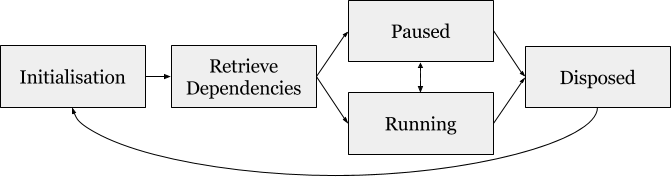
\includegraphics[width=0.7\textwidth]{images/PluginsLifecycle.png}
	\caption{\textit{Rapport Controller}'s plugin's lifecycle.}
	\label{fig:pluginLifecycle}
\end{figure}

After initialisation, the plugins can be either running or paused depending on the state of the \textit{Rapport Controller}. If the controller is running, then \textit{Perceivers} capture external world stimuli and notify the \textit{Effectors} which will attempt to modify the agent's behaviour concurrently by proposing actions asynchronously to the \textit{Rapport Controller} (perceptions events are sent asynchronously but \textit{Effectors} may pool the state of the interaction). The list of active plugins may be changed, either manually by the researcher using the provided \ac{GUI} (Figure~\ref{fig:pluginList}), either automatically by an \textit{Effector} plugin. In any case, in the case of an error in any state transition, the responsible plugin is automatically deactivated and disposed of without escalating to a sudden application crash. Finally, if an error occurs, the researcher is notified with the complete description of the fault.

\begin{figure}[H]
	\centering
	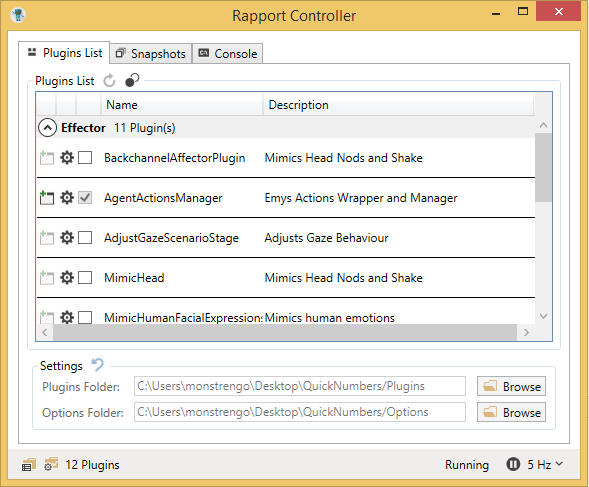
\includegraphics[width=0.6\textwidth]{images/PluginsList.png}
	\caption{\ac{GUI} representation of the list of available plugins.}
	\label{fig:pluginList}
\end{figure}

\subsection{Managing Actions}
\label{sub:sec:managingActions}

The \textit{Rapport Controller} manages action proposals as described in Section~\ref{sec:rapportController} in Chapter~\ref{chap:rapportModel}. However, in addition to the elements of action proposal quintuple $A=<G,P,E,I,T>$, the controller stores the following information:
\begin{itemize}
	\item \textbf{Status}: \textit{pending}, \textit{executing}, \textit{executed} or \textit{interrupted};
	\item \textbf{Starting time}: when the action has started executing;
	\item \textbf{\textit{Thalamus} identifier}: to monitor when actions have finished by monitoring the \textit{Thalamus} messages sent by \textit{Nutty Tracks} and \textit{Speech Server}.
\end{itemize}

The status field is required to manage the state of each action proposal. For example, following Figure~\ref{fig:actionProposalStatus}, an action proposal is only executed (using execution description $E$) as long as its previous state was \textit{pending} and, only then it can be interrupted (using the interruption description $I$). In the absence of the \textit{Thalamus} identifier, we could not flag the actions has executed, making them transition automatically to the \textit{interrupted} state. Furthermore, the controller's default frequency is 10Hz, i.e., the action proposals are analysed 10 times per second.

\begin{figure}[H]
	\centering
	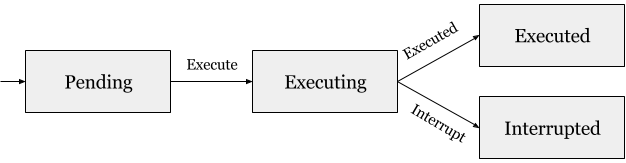
\includegraphics[width=0.6\textwidth]{images/ActionProposalCycle.png}
	\caption{Action Proposal available states and the corresponding transition graph.}
	\label{fig:actionProposalStatus}
\end{figure}

The execution and the interruption descriptions of the action proposal ($E$ and $I$, respectively) are self-contained functions specified by the researcher, therefore they can contain additional logic that is only processed when transitioning to the \textit{executing} state or to the \textit{interrupted} state, respectively. However, in order to change the agent's behaviour, they have to send the required \textit{Thalamus} messages: \textit{Speech Server} to produce utterances or \textit{Nutty Tracks} to trigger animations.

To sum up, the \textit{Effector Plugins} propose actions specifying its priority, how it should be executed, and can additionally specify how the action can be interrupted. The researcher can use the provided \ac{GUI} to debug the proposals as illustrated in Figure~\ref{fig:controllerSnapshots}. Above all, pilots are required to specify the optimal configuration of actions and their priority so that the agent's behaviour satisfies the scenario goals. 

\begin{figure}[H]
	\centering
	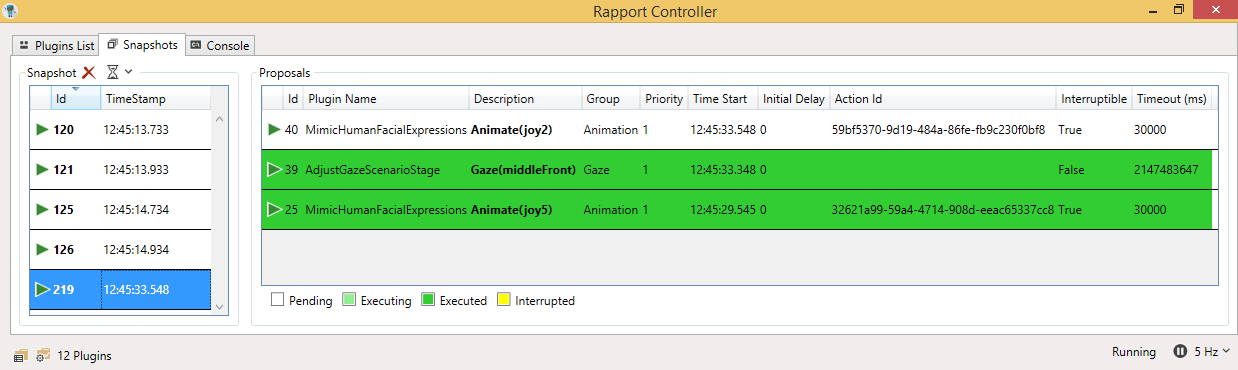
\includegraphics[width=\textwidth]{images/ScreenshotSnapshots.png}
	\caption{\ac{GUI} representation of the snapshots retrieved periodically by the \textit{Rapport Controller}.}
	\label{fig:controllerSnapshots}
\end{figure}